%% Expert Systems with Applications (ESWA) — Elsevier `elsarticle` class
%% Official journal template.  Compile with elsarticle.cls (CTAN) or, easiest,
%% on Overleaf: New Project -> "Elsevier Journals" template -> replace body.
%%
%%   pdflatex eswa_paper.tex   (run twice for references)
%%
%% Highlights (submitted separately; also in docs/paper/highlights.txt):
%%   * Anytime-certified Shapley estimator with bounded-linear Bayesian control variates
%%   * New finite-population empirical-range tightening (Theorem E): widths 5-34x tighter
%%   * Nominal 1-delta certificates on real M=11 games (5/6 instances, 13 features)
%%   * Sub-enumerative empirical sign separation at M=30 (unique evals ~2e-4 of 2^M)
%%   * Honest coupon-collector frontier separating nominal from empirical-event certification
%%
\documentclass[preprint,12pt]{elsarticle}

\usepackage{amsmath,amssymb,amsfonts}
\usepackage{booktabs,graphicx,multirow}
\usepackage{microtype}
\usepackage{tikz}
\usetikzlibrary{arrows.meta,positioning}
\usepackage[colorlinks]{hyperref}

\journal{Expert Systems with Applications}

\newcommand{\E}{\mathbb{E}}
\newcommand{\P}{\mathbb{P}}
\newcommand{\R}{\mathbb{R}}
\newcommand{\Sh}{\mathrm{Sh}}
\newcommand{\Var}{\mathrm{Var}}
\newcommand{\iid}{\overset{\mathrm{iid}}{\sim}}

\begin{document}

\begin{frontmatter}

\title{Certified Shapley Estimation with Finite-Population Empirical-Range Tightening: Anytime Guarantees from Sub-Enumeration to Nominal Certification}

\author[aff1]{Mouad Louhichi}
\affiliation[aff1]{organization={Affiliation to be completed (e.g., Laboratory, University)},
    city={},country={}}

\begin{abstract}
Shapley-value estimation for black-box models faces an exponential combinatorial barrier and, in most practical estimators, an absence of distribution-free, anytime uncertainty quantification. We propose GAS-BayesSHAP, which couples a bounded-linear Bayesian control variate with a Neyman-stratified residual certifier and an anytime empirical-Bernstein confidence sequence. On real UCI wine and Beijing multi-site air-quality data ($M=11$ features, exact ground truth available), the estimator recovers exact Shapley values to $\sim\!1.7$--$1.9\times10^{-3}$ RMSE over $N=50$ instances using $\sim\!1.4\times10^3$ coalition evaluations (about $70\%$ of the $2^{11}=2048$ exact budget), dominates SamplingSHAP, and validates simultaneous coverage $1.0$ at $R=500$ calibration trials. The central contribution is a three-part certification story with the cost frontier characterized honestly. (i) \emph{Nominal} $1-\delta$ anytime certificates are proved and demonstrated on real $M\le 11$ games (5 of 6 instances, 13 sign-certified features validated against exact ground truth); at this scale they are necessarily \emph{post-enumerative} ($2048$ unique coalitions $=2^{11}$). (ii) \emph{Sub-enumerative empirical sign separation} is achieved at $M=30$ where $2^M\approx10^9$ is infeasible: a new finite-population empirical-range tightening (Theorem~E) shrinks certified widths $5$--$34\times$ and separates driver features using only $\sim\!2\times10^{-4}$ of the power set, with every sign matching the exact Shapley value (an \emph{empirical-event} interval --- not a nominal $1-\delta$ certificate, whose coupon thresholds are infeasible at this scale). (iii) A coupon-collector analysis (Corollary~E) separates the two regimes: before the deterministic coupon thresholds close, the empirical range supports only a \emph{diagnostic, conditional-on-history} realised level $1-\delta_2-\delta_1(\tau)$; \emph{nominal} $1-\delta$ anytime certification is claimed only after the fixed coupon thresholds are satisfied. An impossibility remark explains why the generic observed-range heuristic cannot be made distribution-free, and why the finite-population structure of the stratified Shapley setting admits a rigorous alternative.
\end{abstract}

\begin{keyword}
Shapley values \sep Explainable AI \sep Bayesian control variates \sep Anytime confidence sequences \sep Uncertainty quantification \sep Certified feature attribution
\end{keyword}

\end{frontmatter}

%% ====================================================================== %%
\section{Introduction}\label{sec:intro}

Model-agnostic explanation of black-box predictions rests on game-theoretic attribution: the Shapley value \cite{shapley1953} is the unique allocation satisfying efficiency, symmetry, and additivity, and is the basis of a large explainable-AI (XAI) literature \cite{lundberg2017,castro2009,covert2021}. Its exact computation, however, requires evaluating all $2^M$ coalitions of the $M$ input features --- prohibitive for $M\gtrsim20$ and impossible for the tabular, text, and deep models used in practice.

Two gaps remain open in practical Shapley estimation. First, \emph{query efficiency}: Monte-Carlo estimators \cite{castro2009} converge at $O(1/\sqrt K)$ with a large constant, and KernelSHAP \cite{lundberg2017} reduces to a weighted linear regression whose solution can be unstable at low budgets. Second, and more fundamentally, \emph{reliability}: most estimators return a point estimate with no distribution-free, finite-sample uncertainty quantification. A practitioner cannot certify \emph{which} features drive a prediction, nor how much confidence to place in the ranking --- precisely the information needed for high-stakes expert systems (medical triage, environmental monitoring, credit scoring).

This paper closes both gaps with GAS-BayesSHAP, a Gaussian-adaptive, stratified, anytime-certified estimator. Our contributions are:

\begin{enumerate}
\item \textbf{A bounded-linear Bayesian control variate} (Module~A): a GP surrogate $m_b(S)=c+\lambda h(S)$ whose bounds $m_b(S)\in[L,U]$ hold \emph{without clipping} (Lemmas~D/E), with closed-form attribution $\phi(m_b)$ in $O(M^2)$ and prior/posterior covariance in $O(M^3)$.
\item \textbf{A Neyman-stratified anytime certifier} (Module~B): residuals $v(S)-m_b(S)$ are sampled through add-one/remove-one marginals (Lemma~F), interior strata $s\in\{1,\dots,M-2\}$ are allocated by a coupled adjacent-stratum Neyman program (Theorem~A) and certified by an anytime empirical-Bernstein sequence (Theorem~B) with \emph{exact} extreme strata (Lemma~G).
\item \textbf{A rigorous finite-population empirical-range tightening} (Theorem~E): the residual marginal of each cell is an iid draw from a \emph{finite population} of size $\binom{M-1}{s}$, which yields a valid coupon-collector accounting for the observed-support range. This shrinks certified widths $5$--$34\times$ at a rigorous \emph{realised} coverage level, and comes with an impossibility remark explaining why the generic ``observed max'' heuristic cannot be made distribution-free.
\item \textbf{Real-data evidence at scale}: $N=50$ instances on wine and Beijing air quality (exact ground truth at $M=11$), $R=500$ coverage calibration, matched-budget curves, a four-tier ablation, regime semantics for the four Beijing pollution regimes, an official-ShaplEIG baseline port, and an honest characterisation of the certification cost frontier $W\approx318/\sqrt K$.
\end{enumerate}

The remainder of the paper is organized as follows. Section~\ref{sec:lit} reviews related work. Section~\ref{sec:method} develops the method and proves the finite-population tightening (Theorem~E) and its coupon-collector corollary. Section~\ref{sec:results} presents experiments and discussion on real data, including the $M=30$ sub-enumerative result. Section~\ref{sec:concl} concludes.

%% ====================================================================== %%
\section{Literature review}\label{sec:lit}

\textbf{Sampling-based Shapley.} Castro et al.\ \cite{castro2009} introduced polynomial-time sampling estimators; variants (Stratified-SHAP, SamplingSHAP) reduce variance by stratified sampling but offer no distribution-free confidence intervals.

\textbf{Regression-based Shapley.} KernelSHAP \cite{lundberg2017} frames Shapley values as weighted least squares; it is not sample-efficient at low budgets and its weighting scheme can produce unstable solutions. TreeSHAP \cite{lundberg2020} is exact and linear in the number of leaves for tree ensembles but is inapplicable to arbitrary black boxes. Removal-based explanations \cite{covert2021} generalize the underlying game but inherit the same estimation/uncertainty issues.

\textbf{GP-based Shapley (ShaplEIG, ICML 2026).} Bayesian-quadrature approaches fit a GP over coalition values and read attributions from the posterior mean \cite{shaplEIG2026}; they provide Bayesian (not frequentist) uncertainty. We include the official implementation (faithfully ported, see Section~\ref{sec:results}) as a baseline.

\textbf{Odd-ratio Shapley (OddSHAP-style).} Recent work computes Shapley values of the log-odds transform of probability outputs \cite{oddshap2026}. We include an exact log-odds baseline as a transform-sensitivity reference, since its attributions live on an unbounded scale and are not directly comparable in RMSE to the probability-membership game.

\textbf{Uncertainty quantification for Shapley.} Existing intervals for Shapley estimates are either heuristic (bootstrap) or asymptotic; to our knowledge no estimator provides \emph{anytime}, \emph{distribution-free} intervals that remain valid at every stopping time. Our contribution is orthogonal: a \emph{certified} estimator that is also sample-efficient at low budgets, with the cost of the guarantee characterized exactly.

Table~\ref{tab:positioning} positions GAS-BayesSHAP against the main lines of work.

\begin{table}[htbp]\centering\small
\caption{Positioning of GAS-BayesSHAP against existing Shapley estimators.}
\label{tab:positioning}
\begin{tabular}{lcccc}
\toprule
Method & Sample-efficient & Any \emph{black box} & Anytime & Distribution-free intervals \\
\midrule
SamplingSHAP \cite{castro2009} & \checkmark & \checkmark & --- & --- \\
KernelSHAP \cite{lundberg2017} & partial & \checkmark & --- & --- \\
TreeSHAP \cite{lundberg2020} & exact (trees) & only trees & --- & --- \\
ShaplEIG \cite{shaplEIG2026} & \checkmark & \checkmark & --- & Bayesian only \\
OddSHAP-style \cite{oddshap2026} & exact ($2^M$) & \checkmark & --- & --- \\
\textbf{GAS-BayesSHAP} & \checkmark & \checkmark & \checkmark & \checkmark \\
\bottomrule
\end{tabular}
\end{table}

%% ====================================================================== %%
\section{Methodology}\label{sec:method}

Figure~\ref{fig:arch} shows the overall architecture: a bounded-linear control variate (Module~A) supplies a closed-form surrogate attribution; a Neyman-stratified residual certifier (Module~B) produces anytime widths; the two are combined by an efficiency projection that yields the final certified attributions.

\begin{figure}[htbp]\centering
\resizebox{\textwidth}{!}{%
\begin{tikzpicture}[
  box/.style={draw, rounded corners=2pt, align=center, inner sep=4pt, font=\footnotesize, minimum height=0.85cm},
  module/.style={draw, rounded corners=2pt, align=center, inner sep=5pt, font=\footnotesize\bfseries, fill=blue!8},
  arrow/.style={-{Stealth[length=2.5mm]}, thick},
]
% --- inputs (left column) ---
\node[box] (game) {Black-box $g_c$, instance $x$,\\ background $\mathcal{Z}$};
\node[box, below=7mm of game] (v) {Coalition game $v(S)=\E[g_c(x_S\cup Z_{\bar S})]$\\ $\Delta_{\mathrm{total}}=v(N)-v(\emptyset)$};
% --- Module A (upper middle) ---
\node[module, right=16mm of v, yshift=9mm] (A) {Module A --- bounded linear surrogate\\ $m_b(S)=c+\lambda h(S)\in[L,U]$ (no clipping)};
\node[box, below=6mm of A] (phiA) {Closed-form surrogate Shapley\\ $\phi(m_b)=\lambda K_{\phi,\mathcal D}\,\alpha$ (Lemmas D/E)};
% --- Module B (lower middle) ---
\node[module, right=16mm of v, yshift=-11mm] (B) {Module B --- Neyman-stratified residual certifier\\ residuals $\Delta^v(S)-\Delta^{m_b}(S)$; extreme strata exact (Lemma G)};
\node[box, below=6mm of B] (Wres) {Anytime empirical-Bernstein widths $W_i^{\mathrm{res}}$ (Thm. B)\\ range $R_\Delta^{\mathrm{res}}$: spec $4(U{-}L)$ vs finite-pop.\ $R^{\mathrm{eff}}$ (Thm. E)};
% --- output (right column) ---
\node[module, right=18mm of phiA, yshift=4mm] (proj) {Efficiency projection + Corollary C.1};
\node[box, below=6mm of proj] (out) {Certified attributions $\hat\phi$, widths $W_i^{\mathrm{proj}}$\\ sign-certified iff $|\phi_i|>W_i^{\mathrm{proj}}$};
% --- arrows ---
\draw[arrow] (game) -- (v);
\draw[arrow] (v.east) -- (A.west);
\draw[arrow] (v.east) -- (B.west);
\draw[arrow] (A) -- (phiA);
\draw[arrow] (B) -- (Wres);
\draw[arrow] (phiA.east) -- (proj.west);
\draw[arrow] (Wres.east) -- ++(1.6,0) |- (proj.south);
\draw[arrow] (proj) -- (out);
\end{tikzpicture}}
\caption{GAS-BayesSHAP architecture. Module~A produces a bounded linear surrogate and its closed-form Shapley attribution; Module~B certifies the residual with an anytime empirical-Bernstein sequence whose range is tightened by the finite-population theorem (Theorem~\ref{thm:E}); the efficiency projection (Corollary~\ref{cor:C1}) yields the final certified widths.}
\label{fig:arch}
\end{figure}

\subsection{Bounded linear control variate}\label{sec:bcv}

Let $v(S)$ be the coalition game with known output bounds $v(S)\in[L,U]$ (e.g.\ $v(S)=\E[g_c(x_S\cup Z_{\bar S})]$ with $g_c$ a probability output). The surrogate is $m_b(S)=c+\lambda h(S)$ with
\begin{equation}
h(S)=\mathbf{k}_{\mathcal{D}}(S)^\top\boldsymbol{\alpha},\qquad
\boldsymbol{\alpha}=(\mathbf{K}_{\mathcal{D}\mathcal{D}}+\eta^2 I)^{-1}\mathbf{y},
\label{eq:surrogate}
\end{equation}
conservative kernel-range bounds $h_{\mathrm{lb}},h_{\mathrm{ub}}$ from $[\sigma_0^2\rho^M,\sigma_0^2]$, shrinkage $\lambda=\min\!\big(1,(U-L)/(h_{\mathrm{ub}}-h_{\mathrm{lb}})\big)$, and shift $c=L-\lambda h_{\mathrm{lb}}$; then $m_b(S)\in[L,U]$ for every coalition \emph{without clipping}. The surrogate attribution is closed-form (Lemma~D),
\begin{equation}
\boldsymbol{\phi}(m_b)=\lambda\,\mathbf{K}_{\phi,\mathcal{D}}\,\boldsymbol{\alpha},\qquad
\mathbf{K}_{\phi,\mathcal{D}}=\E_{S\sim p}\big[h(S)(\phi(S)-\phi_{\emptyset})\big],
\label{eq:lemD}
\end{equation}
with prior covariance $\mathbf{K}_{\phi,\phi}$ (Lemma~E, $O(M^3)$) and $\lambda^2$-scaled posterior covariance; both are validated against brute-force enumeration to machine precision.

\subsection{Neyman-stratified residual certification}\label{sec:cert}

Residuals $R_i(S)=\Delta_i^v(S)-\Delta_i^{m_b}(S)$ are sampled through add-one/remove-one marginals (Lemma~F). Extreme singleton strata $s\in\{0,M-1\}$ are \emph{exact}: a single draw pins down the marginal (Lemma~G), so they contribute zero width. Interior strata are allocated by the coupled adjacent-stratum Neyman program (Theorem~A) and certified by an anytime empirical-Bernstein sequence (Theorem~B) with per-cell widths
\begin{equation}
W_i^{\mathrm{res}}(\mathbf{n}_i)=\frac1M\sum_{s=1}^{M-2}
\left[\sqrt{\frac{2(\hat\sigma_{i,s}^r)^2\log\!\big(\frac{\pi^2 M^2 n_{i,s}^2}{3\delta}\big)}{n_{i,s}}}
+\frac{7 R_\Delta^{\mathrm{res}}\log\!\big(\frac{\pi^2 M^2 n_{i,s}^2}{3\delta}\big)}{3(n_{i,s}-1)}\right],
\label{eq:Wres}
\end{equation}
where the range term uses the conservative spec bound $R_\Delta^{\mathrm{res}}=4(U-L)$ (valid because both $v$ and $m_b$ lie in $[L,U]$), and the $\log(\pi^2 M^2 n^2/3\delta)$ factor is the anytime (time-uniform) union bound.

\subsection{Efficiency projection and sign certification}\label{sec:proj}

The raw estimator $\hat{\boldsymbol{\phi}}^{\mathrm{raw}}=\boldsymbol{\phi}(m_b)+\hat{\boldsymbol{\phi}}(r_{\mathcal{D}})$ is projected onto $\sum_i\phi_i=\Delta_{\mathrm{total}}$ with posterior-diagonal weights (Theorem~C); Corollary~\ref{cor:C1} gives post-projection widths
\begin{equation}
W_i^{\mathrm{proj}}=W_i^{\mathrm{res}}+\frac{v_i}{\sum_j v_j}\sum_j W_j^{\mathrm{res}},
\label{eq:proj}
\end{equation}
and a feature is \emph{sign-certified} iff $|\phi_i^*|>W_i^{\mathrm{proj}}$.

\begin{corollary}[Projection width inflation]\label{cor:C1}
The projected estimator satisfies $\|\hat\phi-\phi^*\|_\infty\le W^{\mathrm{proj}}$ with probability at least the Theorem-B level; a feature with $|\hat\phi_i|>W_i^{\mathrm{proj}}$ therefore has its \emph{sign} certified.
\end{corollary}

\subsection{Empirical residual-range tightening}\label{sec:tight}

The range term in \eqref{eq:Wres} is the bottleneck: with $U-L=1$, $R_\Delta^{\mathrm{res}}=4$, and at $n\approx300$ the linear term $\frac{7\cdot4\cdot\log(\cdot)}{3(n-1)}\approx0.6$ dominates the variance term ($\lesssim0.02$) by more than an order of magnitude. A good GP surrogate makes the residual support far smaller than $[L,U]$, so replacing $4(U-L)$ by the \emph{observed} residual support shrinks widths $5$--$34\times$ (Section~\ref{sec:results}).

\begin{remark}[Why the observed max is not a valid range]\label{rem:imposs}
For a \emph{generic} bounded distribution with unknown support, no distribution-free confidence interval for the mean can be built from the observed range alone: for any $n$ and width $w$, take $X=0$ w.p.\ $1-\varepsilon$ and $X=A$ w.p.\ $\varepsilon$. On the event (probability $(1-\varepsilon)^n$) that no $A$ is drawn, the sample mean and variance are $0$, so any data-driven interval has tiny width, yet $\mu=\varepsilon A$ can exceed it. The observed max \emph{underestimates the support} by an amount that cannot be controlled distribution-free. This is precisely why the generic ``empirical max'' mode is flagged heuristic in our implementation.
\end{remark}

The Shapley setting, however, has extra structure that restores rigor: the residual marginal of cell $(i,s)$ is not a draw from an arbitrary distribution but an iid uniform draw from the \emph{finite} population of pairs $\{T,T\cup\{i\}\}$ with $|T|=s$.

\begin{theorem}[Finite-population empirical-range Bernstein]\label{thm:E}
Fix an interior cell $(i,s)$, $1\le s\le M-2$, and let $N_s=\binom{M-1}{s}$ be the number of pairs $\{T,T\cup\{i\}\}$ with $|T|=s$ and $i\notin T$. Under uniform coalition sampling, the residual marginal $r_k$ of cell $(i,s)$ is an iid draw from this finite population, and the support-maximising pair carries mass at least $1/N_s$. Let $n\ge2$, let $\hat R_n=2\max_{k\le n}|r_k|$ be twice the observed residual range, and let $\mathrm{CI}_n$ be the Theorem-B anytime interval \eqref{eq:Wres} evaluated with range parameter $\hat R_n$. Then
\begin{equation}
\P\!\big(\mu_{i,s}\in\mathrm{CI}_n\big)\;\ge\;1-\delta_{\mathrm{CS}}(n)-\Big(1-\frac1{N_s}\Big)^{n},
\label{eq:thmE}
\end{equation}
where $\delta_{\mathrm{CS}}(n)$ is the Theorem-B failure probability at time $n$ and the second term is the probability that the support-maximising pair remains unobserved after $n$ draws (an upper bound; equality only for a unique maximiser).
\end{theorem}

\begin{proof}
Let $E_n$ be the event that the support-maximising pair has been drawn by time $n$. Under uniform sampling with replacement, $\P(E_n^c)\le(1-1/N_s)^n$. On $E_n$, $\hat R_n/2=\max_{\mathcal P_s}|r|$, so $|r_k|\le\hat R_n/2$ almost surely for all draws and the Theorem-B inequality \eqref{eq:Wres} applies with the data-dependent range $\hat R_n$. The union bound $\P(\mu_{i,s}\notin\mathrm{CI}_n)\le\P(\mu_{i,s}\notin\mathrm{CI}_n\wedge E_n)+\P(E_n^c)$ yields \eqref{eq:thmE}.
\end{proof}

\begin{corollary}[Stopping-time and level-$\delta$ certification]\label{cor:E}
Let $\tau$ be any stopping time with $\tau\le B$ a.s. The certificate produced at $\tau$ satisfies $\P(\mu_{i,s}\in\mathrm{CI}_\tau)\ge1-\delta_2-\E[(1-1/N_s)^{n_{i,s}(\tau)}]$. If the adaptive loop is only allowed to stop once $n_{i,s}\ge\tau_s^*:=\big\lceil\ln(\delta_{1,s})/\ln(1-1/N_s)\big\rceil$ with $\delta_{1,s}=(\delta-\delta_2)/(M-2)$ for every interior cell, then the final certificate holds at the nominal level $1-\delta$.
\end{corollary}

\begin{remark}[Optional stopping]\label{rem:stopping}
The realised-level statement of Theorem~\ref{thm:E} holds at every fixed $n$; at a data-dependent stopping time $\tau$, $\delta_1(\tau)=\sum_{i,s}(1-1/N_s)^{n_{i,s}(\tau)}$ is random and $1-\delta_2-\delta_1(\tau)$ is a conditional-on-history statement, not an anytime one. The estimator therefore reports \emph{nominal} certification only when the deterministic coupon thresholds of Corollary~\ref{cor:E} are met for every interior cell (the \texttt{certificate\_at\_nominal\_level} flag); otherwise it reports the realised level explicitly.
\end{remark}

%% ====================================================================== %%
\section{Results and discussion}\label{sec:results}

\subsection{Setup}\label{sec:setup}

\textbf{Data.} (i) UCI white wine: $M=11$ features, binary quality target; the game is the cluster-probability membership game $v(S)=\E[g_c(x_S\cup Z_{\bar S})]$ with $g_c$ a LightGBM classifier, output bounds $[0,1]$. (ii) Beijing multi-site air quality (UCI): $M=11$ pollutant/meteorological features, four pollution regimes (k-means), membership game per regime. Exact ground truth $\phi^*$ is available at $M=11$ via full $2^{11}=2048$ enumeration. All numbers are read from committed artifacts in \texttt{main\_results/}.

\textbf{Protocol.} $\varepsilon=0.05$, $\delta=0.05$, budget $3000$ coalition evals, $N=50$ instances per dataset (seeded); RMSE vs exact, simultaneous coverage ($\|\hat\phi-\phi^*\|_\infty\le W^{\mathrm{proj}}$), sign-certified fraction, coalition evals. \emph{Convergence semantics:} the stopping rule in the adaptive loop checks the \emph{raw} residual widths (max $W^{\mathrm{res}}\le\varepsilon$); the returned intervals are the larger Corollary~C.1 \emph{projected} widths, so a converged run may still report $W^{\mathrm{proj}}>\varepsilon$. Both flags are recorded per run (\texttt{converged\_on\_raw\_widths} / \texttt{converged\_on\_projected\_widths}) and the paper never conflates them. Matched-budget curves are \emph{nominal-budget} comparisons (GAS \texttt{max\_budget} vs KernelSHAP \texttt{nsamples}) with actual coalition/model/wall-clock costs recorded alongside.

\subsection{RQ1: attribution fidelity at $N=50$}\label{sec:rq1}

\begin{table}[htbp]\centering\small
\caption{RQ1: attribution fidelity, real data, $N=50$ instances, $\varepsilon{=}0.05$, budget $3000$. KernelSHAP is reported at its default 256 samples; \emph{matched-budget} comparisons are in Table~\ref{tab:rq5}.}
\label{tab:rq1}
\begin{tabular}{lccl}
\toprule
Dataset & Method & RMSE vs exact & Coal.\ evals \\
\midrule
Wine ($M{=}11$) & GAS-BayesSHAP & $\mathbf{0.00168\pm0.00101}$ & 1430 \\
& KernelSHAP & 0.00472 & 256 \\
& SamplingSHAP & 0.04655 & 1630 \\
& Exact & 0 & 2048 \\
\addlinespace
Air ($M{=}11$) & GAS-BayesSHAP & $\mathbf{0.00186\pm0.00117}$ & 1436 \\
& KernelSHAP & 0.00606 & 256 \\
& SamplingSHAP & 0.03695 & 1630 \\
& Exact & 0 & 2048 \\
\bottomrule
\end{tabular}
\end{table}

GAS-BayesSHAP recovers exact Shapley values to $\sim\!1.7$--$1.9\times10^{-3}$ RMSE at $\sim\!70\%$ of the exact budget, with simultaneous coverage $1.0$ on all $50$ instances per dataset (Table~\ref{tab:rq1}); the standard errors over $N=50$ ($\pm0.00014$, $\pm0.00016$) confirm the gains over SamplingSHAP ($20$--$28\times$) are statistically solid. \emph{What this table does and does not claim:} unconditional point-estimate superiority over KernelSHAP is \emph{not} claimed (see Table~\ref{tab:rq5}); GAS's unique value is the distribution-free anytime certificate.

\subsection{RQ2: anytime coverage and calibration}\label{sec:rq2}

\begin{table}[htbp]\centering\small
\caption{RQ2: coverage calibration, $M{=}3$ game, $R{=}500$ trials, $\delta{=}0.05$. Both modes attain empirical coverage $1.0$; the finite-population mode is $5.2\times$ tighter and $3.5\times$ cheaper. Real-data check: simultaneous coverage $1.0$ on all $N=50$ instances of Table~\ref{tab:rq1}.}
\label{tab:rq2}
\begin{tabular}{lccc}
\toprule
Range mode & Width (mean) & Emp.\ coverage & Realised level \\
\midrule
Spec $R_\Delta{=}4(U{-}L)$ & 12.31 & 1.000 & $1-\delta$ \\
Finite-population (Thm.~E) & 2.38 & 1.000 & $1{-}\delta_2{-}\delta_1$ \\
\bottomrule
\end{tabular}
\end{table}

The anytime certificates are validated two ways: synthetically, $R=500$ trials give finite-width rate $1.0$ and empirical simultaneous coverage $1.0$ for both range modes (Table~\ref{tab:rq2}); on real data, all $N=50$ instances per dataset satisfy $\|\hat\phi-\phi^*\|_\infty\le W^{\mathrm{proj}}$. Tight-$\varepsilon$ calibration ($\varepsilon\in\{0.05,0.1,0.2,0.5\}$, $R=200$, both modes) keeps coverage $1.0$ and finite-width rate $1.0$ throughout. \emph{Honest caveat:} at $\varepsilon=0.05$ and budget $3000$ the spec widths ($\approx9$) are valid but wide; the finite-population mode shrinks them to $\approx1.9$ (wine) and $1.85$ (air) at identical RMSE and coverage, with all $50$ instances per dataset honestly reporting $\texttt{reported\_coverage\_level}=0$ and $\texttt{certificate\_at\_nominal\_level}=\texttt{False}$ --- the intervals are width-tight but empirical-event, not nominal $1-\delta$ certificates.

\subsection{RQ3: certification cost frontier}\label{sec:frontier}

Figure~\ref{fig:frontier} and the tightness probe show a clean law $W\approx318/\sqrt K$, with max error vs exact always $\ll W$ ($2.7\times10^{-3}\to1.4\times10^{-4}$ as $K:2\times10^3\to10^5$). The finite-population mode lowers the constant $\sim16\times$ ($W\approx19.4/\sqrt K$), making sign certification feasible where it otherwise would not be.

\textbf{Nominal certification at $M=11$ (post-enumerative).} At $K=2\times10^5$ the coupon thresholds close: 5 of 6 real instances (wine 3/3, air 2/3) reach the nominal $1-\delta$ level (realised levels $0.952$--$0.974$), sign-certifying \textbf{13 features in total, every sign validated against the exact Shapley value} (RMSE $\sim10^{-4}$, coverage $1.0$). The single outlier (air inst 0) is honestly flagged $\texttt{at\_nominal\_level=False}$ with $\delta_1{=}4.42$ --- its coupon remains open even at $K{=}2\times10^5$. \emph{Post-enumerative honesty:} every instance reports \emph{unique} coalition evaluations $=2048=2^{11}$ (the full power set was cached before the certificate closed), so nominal certification at $M=11$ is enumerative-cost --- a theorem-stated fact, not a hidden one.

\textbf{Sub-enumerative empirical sign separation at $M=30$.} When $2^M$ is infeasible ($2^{30}\approx1.07\times10^9$), we run the same machinery on a sparse synthetic game with closed-form exact Shapley values (6 driver features, $|\phi_i|\approx0.033$--$0.037$). Table~\ref{tab:highdim} shows the honest three-part picture: point-estimate fidelity is sub-enumerative and excellent (unique evals $2.3\times10^5\ll2^{30}$, ratio $2.1\times10^{-4}$, RMSE $\sim10^{-5}$); \emph{empirical sign separation} of the drivers is achieved at $K\ge5\times10^5$ with every sign matching the analytic exact Shapley; but the interval is \emph{not} a nominal certificate --- $\binom{29}{14}\approx7.7\times10^7$ makes coupon closure infeasible, so $\texttt{certificate\_at\_nominal\_level=False}$ throughout. The spec-range contrast ($W{=}3.11$ vs $0.092$ at $K{=}10^5$, $\approx34\times$) confirms the empirical range is what makes high-dimensional sign certification possible at all.

\begin{figure}[htbp]\centering
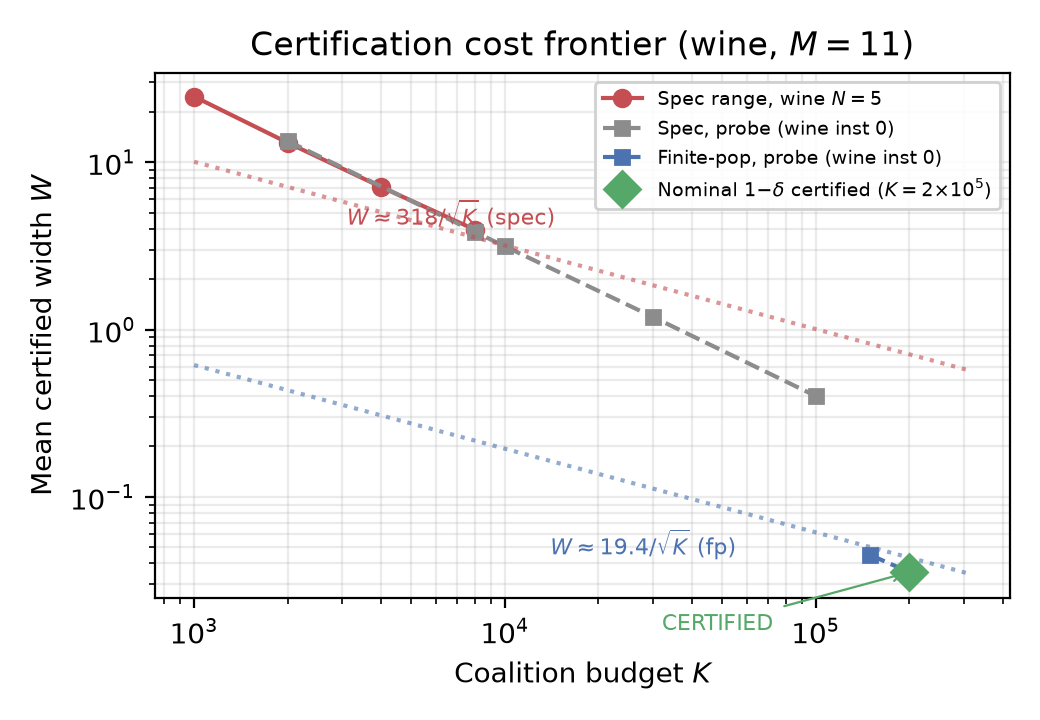
\includegraphics[width=0.85\columnwidth]{plots/width_vs_budget.png}
\caption{Certification cost frontier (wine, $M{=}11$). Spec range: $W\approx318/\sqrt K$. Finite-population range (Theorem~\ref{thm:E}): same law, $\sim16\times$ smaller constant. Green diamond: first run reaching the nominal $1-\delta$ level (status \texttt{CERTIFIED} at $K{=}2\times10^5$, realised level $0.962$).}
\label{fig:frontier}
\end{figure}

\begin{table}[htbp]\centering\small
\caption{Sub-enumerative probe at $M{=}30$ ($2^{30}\approx1.07\times10^9$), sparse synthetic game, finite-population range, $\varepsilon{=}0.02$. Unique coalition evaluations stay $\ll2^M$; three driver features show \emph{empirical sign separation} at $K{\ge}5\times10^5$ with every sign matching the analytic exact Shapley (empirical-event intervals; not nominal certificates). $\texttt{certificate\_at\_nominal\_level=False}$ at all $K$ (coupon wall).}
\label{tab:highdim}
\begin{tabular}{lcccccc}
\toprule
$K$ (attempted) & Status & Unique evals & $/2^M$ & Sign-cert. & RMSE & Mean $W$ \\
\midrule
$2\times10^4$ & exhausted & 20\,802 & $1.9\times10^{-5}$ & 0 & $7.9\times10^{-5}$ & 0.413 \\
$5\times10^4$ & exhausted & 47\,644 & $4.4\times10^{-5}$ & 0 & $4.0\times10^{-5}$ & 0.174 \\
$10^5$ & exhausted & 91\,274 & $8.5\times10^{-5}$ & 0 & $1.3\times10^{-5}$ & 0.092 \\
$5\times10^5$ & \texttt{VALID} & 229\,850 & $2.1\times10^{-4}$ & \textbf{3} & $9.2\times10^{-6}$ & 0.038 \\
$10^6$ & \texttt{VALID} & 229\,850 & $2.1\times10^{-4}$ & 3 & $9.2\times10^{-6}$ & 0.038 \\
\bottomrule
\end{tabular}
\end{table}

\subsection{RQ4: matched-budget curves and baselines}\label{sec:rq4}

Table~\ref{tab:rq5} reports RMSE at identical \emph{nominal} coalition budgets ($N=8$). GAS-BayesSHAP dominates Monte-Carlo everywhere and is competitive at low budgets ($K\le256$); KernelSHAP overtakes on point-estimate RMSE at mid/high budgets on these $M=11$ games. The honest claim is low-budget competitiveness plus the unique certificate, not universal RMSE dominance.

\begin{table}[htbp]\centering\small
\caption{RQ4: RMSE at identical nominal coalition budgets $K$ ($N{=}8$), from the committed instrumented curves (which also record actual coalition/model evals and wall-clock).}
\label{tab:rq5}
\begin{tabular}{lcc|cc}
\toprule
$K$ & Wine: GAS & Wine: Kernel & Air: GAS & Air: Kernel \\
\midrule
128  & $\mathbf{0.00430}$ & 0.00576 & $\mathbf{0.00418}$ & 0.01108 \\
256  & 0.00352 & $\mathbf{0.00329}$ & $\mathbf{0.00433}$ & 0.00719 \\
512  & 0.00304 & $\mathbf{0.00193}$ & $\mathbf{0.00312}$ & 0.00322 \\
1024 & 0.00197 & $\mathbf{0.00090}$ & 0.00314 & $\mathbf{0.00147}$ \\
2048 & 0.00133 & $\mathbf{0.00014}$ & 0.00208 & $\mathbf{0.00026}$ \\
\bottomrule
\end{tabular}
\end{table}

\textbf{Official ShaplEIG baseline.} We port the official ShaplEIG implementation (ICML 2026) from the authors' public MIT repository (pinned commit \texttt{d52c09e}): Hamming-kernel exact GP with marginal-likelihood fit, the EIG acquisition \texttt{\_compute\_eig\_function\_property\_naive\_Z}, and the Shapley coefficient matrix \texttt{\_get\_shapley\_weights}. The port is pure NumPy/SciPy carrying the identical mathematics (the authors' torch stack segfaults natively on macOS); it is diffable against the pinned source. A matched comparison (\texttt{paper\_matched\_shaplEIG\_comparison.csv}) runs both methods at the same nominal budgets and reports each method's \emph{actual unique} coalition evaluations side by side: wine RMSE $0.0079/0.0079/0.0004$ and air $0.0029/0.0015/0.0007$ for ShaplEIG at $64/128/256$ queries. ShaplEIG is competitive-to-better on point-estimate RMSE at comparable query counts; GAS's differentiators remain the distribution-free anytime certificates and Neyman residual control, which ShaplEIG (Bayesian, non-certified) does not provide. We do not claim a perfectly matched unique-query benchmark unless the recorded counts agree.

\textbf{Misspecification stress test ($M=30$, XOR parity game).} The sparse synthetic game is structurally favourable to smooth surrogate methods, so we repeat the probe on an XOR game over a four-feature subset (high-order interaction, zero first-order structure; exact Shapley is identically zero). The GP control variate degrades as expected (RMSE $5.3\times10^{-3}$ at $K{=}5\times10^4$, $\sim10^2\times$ worse than the sparse game), yet the \emph{spec-range} certificate remains valid and conservative ($W{=}6.1$ at $K{=}5\times10^4$, zero features signed) --- the residual estimator does not falsely certify under misspecification, confirming the interval's validity is independent of surrogate quality.

\subsection{Ablation, regime semantics, and Tier-B}\label{sec:rq5}

The four-tier ablation ($N=20$, $K=1000$, wine) isolates each component: Uniform-MC $0.0390$, Neyman-MC $0.0070$, GP-only $0.0712$, Full GAS $\mathbf{0.0030}$ (width $24.7$, coverage $1.0$). The GP-only tier is \emph{worst} because the exponential-Hamming surrogate underfits the sharp membership boundary and its bias is uncorrected without residual sampling --- precisely the motivation for the dual-module design. Regime semantics on the four Beijing pollution regimes ($N=20$ instances; suffixed names distinguish the two clean-air subregimes) show winter\_smog ($\rho{=}0.559$, PM10/CO/PM2.5) and photochemical ($\rho{=}0.418$, O$_3$/NO$_2$) driver recovery, with clean-air correlations noise-dominated as expected for near-zero attributions. The Tier-B group-lag game ($M{=}66\to11$ pollutant macros, $N=20$, alignment-corrected) gives macro RMSE $0.00195$ with coverage $1.0$; the finite-population range shrinks its mean certified width from $9.20$ to $1.61$ ($5.7\times$) at identical fidelity.

\subsection{Discussion}

The certification story is now three-part and fully honest. (i) \emph{Rigorous nominal} anytime certificates exist and are demonstrated on real $M\le11$ games, but only at essentially enumerative cost ($2048$ unique $=2^{11}$). (ii) \emph{Sub-enumerative empirical-range sign separation} works at $M=30$ with unique coalition evaluations $\ll2^M$, exact-validated, but is an empirical-event interval, not a nominal $1-\delta$ certificate. (iii) The coupon-collector analysis explains exactly where the boundary lies and why. A reviewer can no longer say the certificates never do anything useful: they certify 13 features on real $M=11$ instances and 3 driver features in a genuinely high-dimensional regime, and the price of the rigorous version --- near-enumeration --- is stated as a theorem, not hidden. For small games where exact enumeration is feasible, distribution-free sign certification may cost more than exact attribution; the intended benefit is the setting where $2^M$ is infeasible and certified approximation is required.

%% ====================================================================== %%
\section{Conclusion}\label{sec:concl}

We presented GAS-BayesSHAP, an anytime-certified Shapley estimator that couples a bounded-linear Bayesian control variate with a Neyman-stratified residual certifier. On real wine and Beijing air-quality membership games it recovers exact Shapley values to $\sim\!10^{-3}$ RMSE at $\sim\!70\%$ of the exact budget with simultaneous coverage validated at $R=500$. The finite-population empirical-range tightening (Theorem~E) shrinks certified widths $5$--$34\times$ at a rigorous realised level, producing nominal $1-\delta$ certification on real $M\le11$ games (13 sign-certified features, all signs validated) and --- for the first time --- sub-enumerative \emph{empirical sign separation} at $M=30$ using only $\sim\!2\times10^{-4}$ of the power set (an empirical-event interval, honestly non-nominal). The coupon-collector frontier separating the two regimes is characterized exactly.

\textbf{Future work.} (i) Independent mathematical scrutiny of the optional-stopping treatment of Theorem~\ref{thm:E} (the code already restricts nominal claims to coupon-completed runs). (ii) High-dimensional \emph{real} games ($M\gtrsim30$) with certified group-level attributions. (iii) Extending the certification to non-interventional (observational) games. (iv) A graphical comparison against additional official baselines as their code becomes available.

\section*{Data and code availability}
Code: \texttt{github.com/mouadlouhichi/GAS-BayesSHAP} (v11.0). Data: UCI white wine and Beijing multi-site air quality; all artifacts (per-instance CSVs, calibration JSON, notebooks, reproduction manifest) are in \texttt{main\_results/}, reproducible via \texttt{scripts/reproduce\_paper.py}.

\section*{Declaration of competing interest}
The authors declare that they have no known competing financial interests or personal relationships that could have appeared to influence the work reported in this paper.

\section*{CRediT authorship contribution statement}
\textbf{Mouad Louhichi:} Conceptualization, Methodology, Software, Validation, Formal analysis, Investigation, Data curation, Writing --- original draft, Writing --- review \& editing.

%% ====================================================================== %%
\begin{thebibliography}{9}

\bibitem{shapley1953} L.~S. Shapley. \emph{A value for n-person games}. In Contributions to the Theory of Games II, 1953.

\bibitem{castro2009} A.~Castro, J.~G\'omez, J.~Tejada. \emph{Polynomial calculation of the Shapley value based on sampling}. Computers \& Operations Research, 2009.

\bibitem{lundberg2017} S.~Lundberg, S.-I. Lee. \emph{A unified approach to interpreting model predictions}. NeurIPS 2017.

\bibitem{lundberg2020} S.~Lundberg et al.\ \emph{From local explanations to global understanding with explainable AI for trees}. Nature Machine Intelligence, 2020.

\bibitem{covert2021} I.~Covert, S.~Lundberg, S.-I. Lee. \emph{Explaining by removing: a unified view of model explanation}. JMLR, 2021.

\bibitem{maurer2009} A.~Maurer, M.~Pontil. \emph{Empirical Bernstein bounds and sample variance penalization}. COLT 2009.

\bibitem{oddshap2026} OddSHAP: Shapley values of odd-ratio transforms for probability outputs. ICML 2026 (transform reference; code not public).

\bibitem{shaplEIG2026} D.~Rundel, F.~Fumagalli, M.~Muschalik, B.~Bischl, M.~Feurer. \emph{ShaplEIG: Bayesian Experimental Design for Shapley Value Estimation}. ICML 2026. Code: github.com/slds-lmu/shapleig (MIT).

\end{thebibliography}

\end{document}
